% graphic source https://docs.google.com/presentation/d/10CJGfUzKqPQKf-JCOsQuNULPU8LJzB31G_NQ8VyVIhg
\begin{figure}
\begin{minipage}{0.65\linewidth}
\begin{subfigure}{0.5\linewidth}
    \captionsetup{labelformat=prependbefore,labelsep=space}
  \includegraphics[height=1.65in]{img/steady-bars}
  \caption{\footnotesize steady policy}
  \label{fig:steady-vs-tilted-schematic:steady}
\end{subfigure}%
\begin{subfigure}{0.5\linewidth}
  \centering
  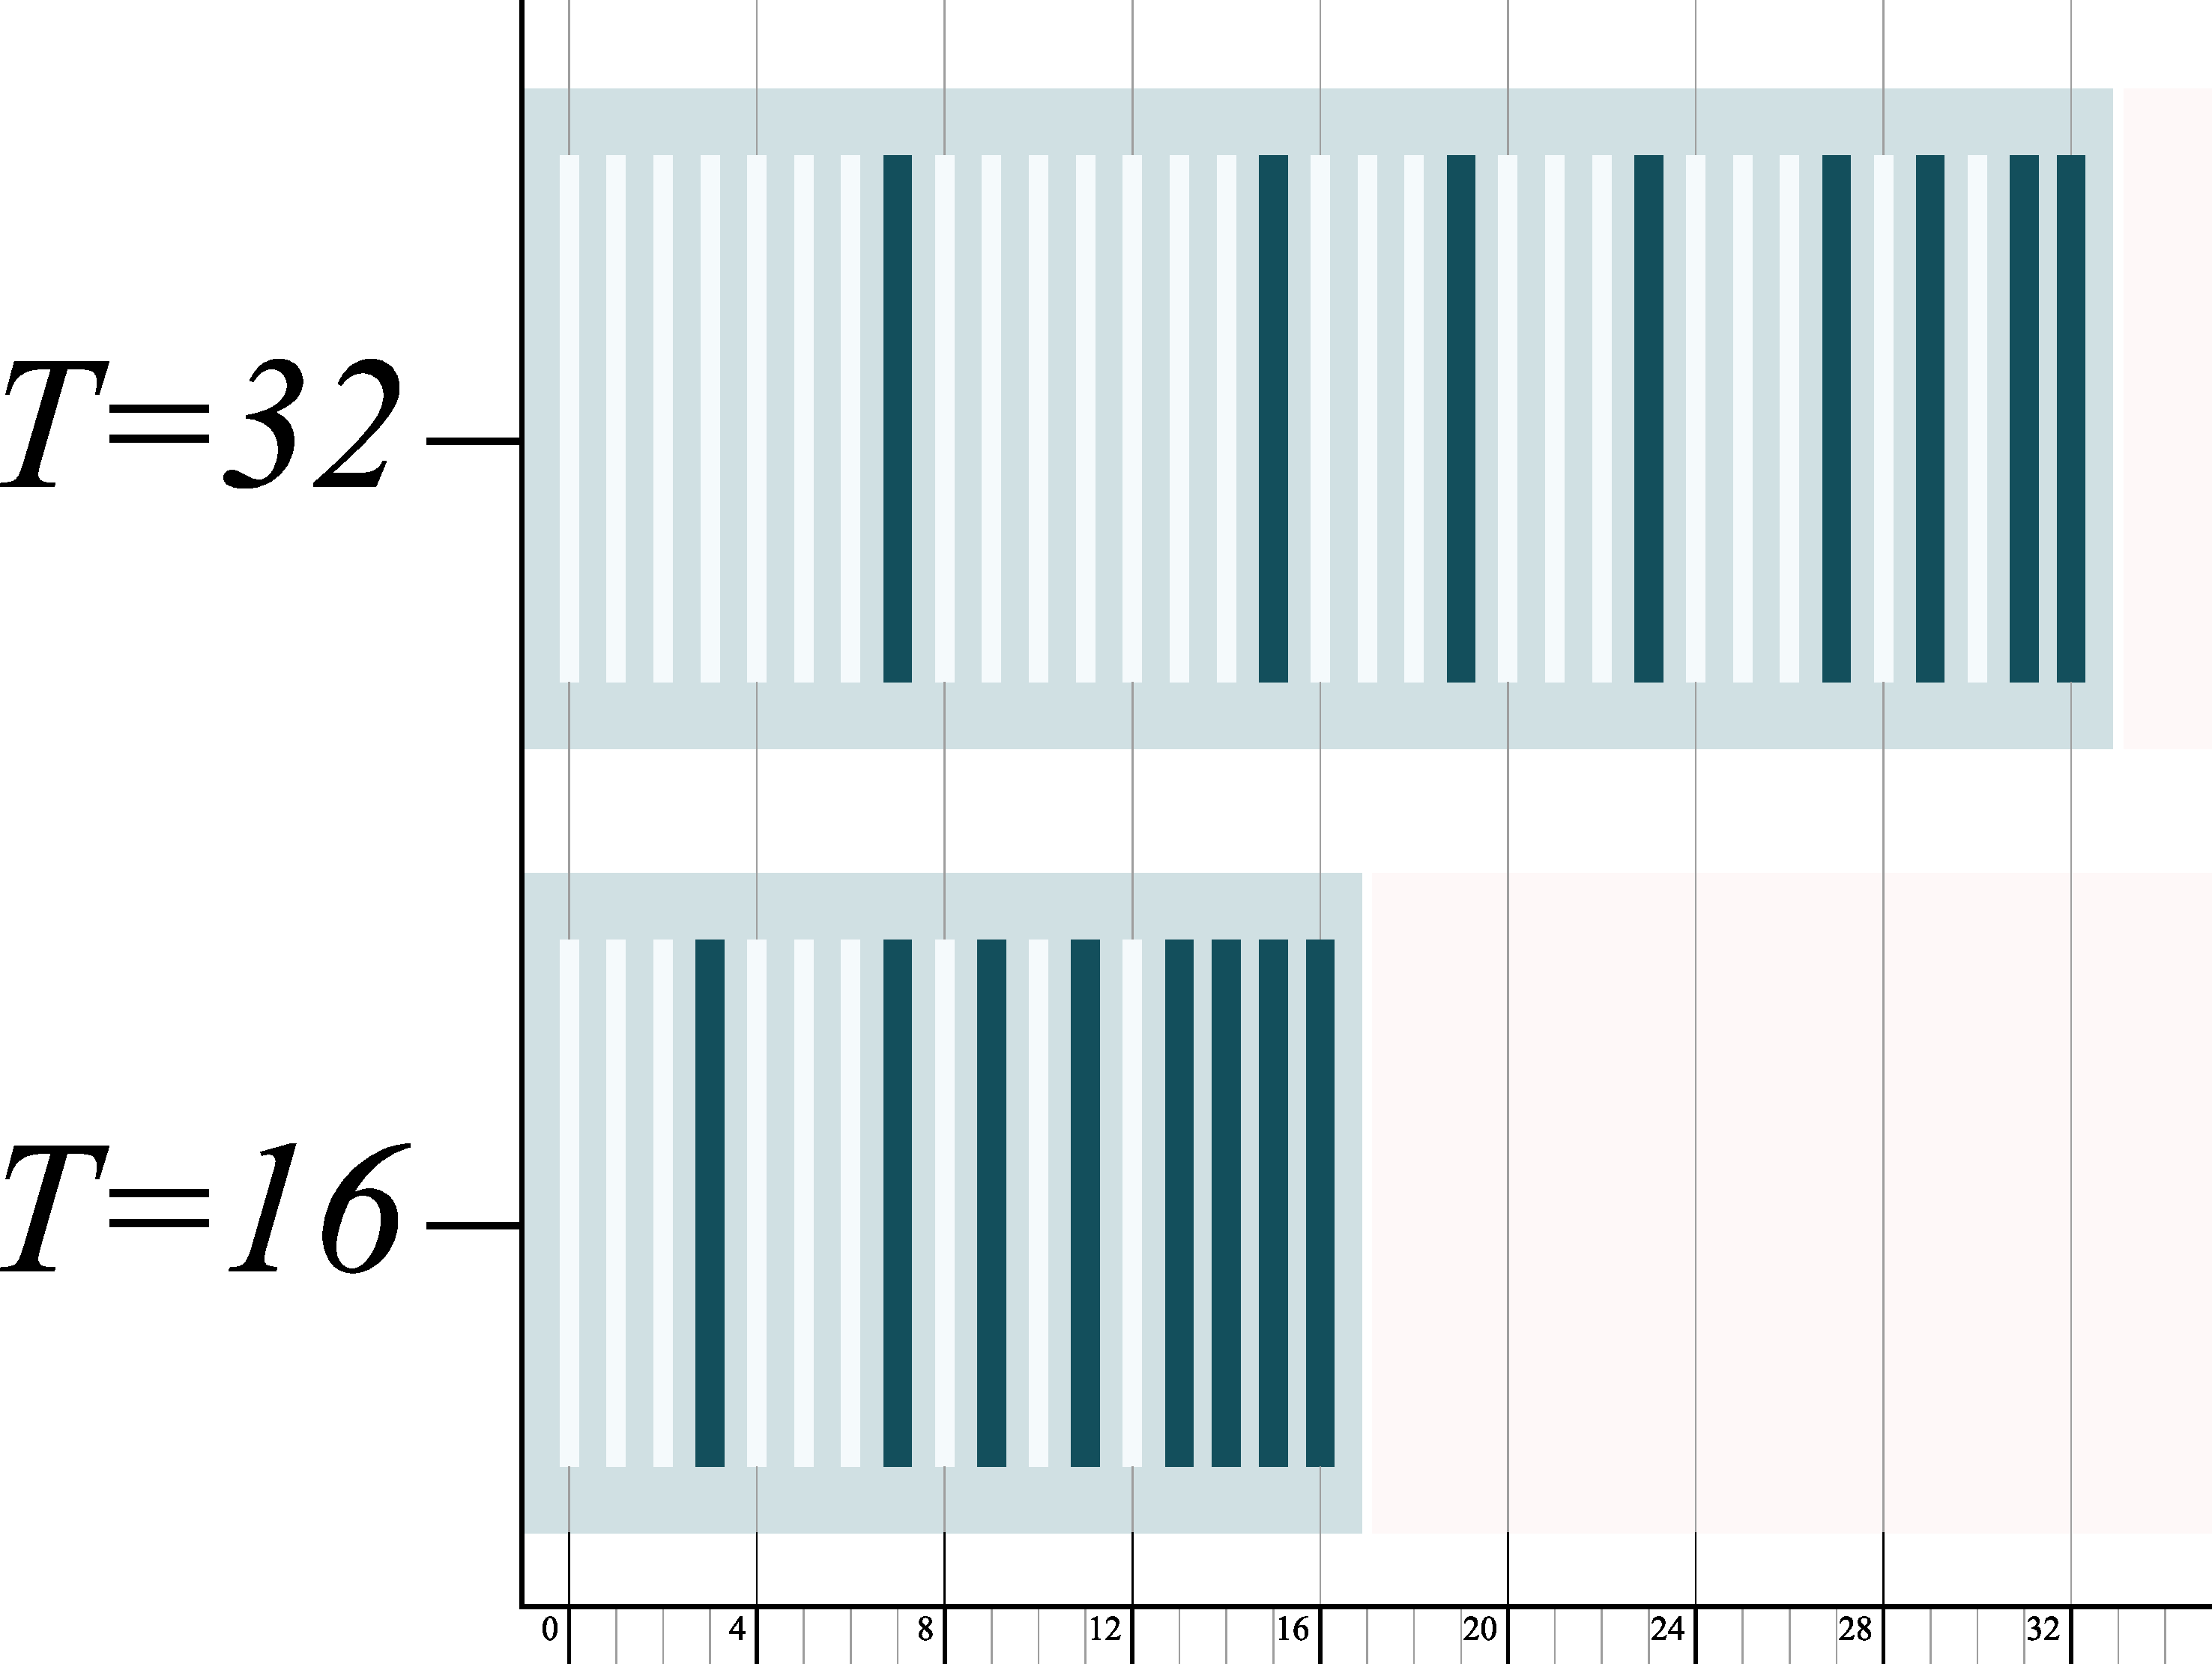
\includegraphics[height=1.65in, trim={10cm 0 0 0}, clip]{img/tilted-bars}
  \caption{\footnotesize tilted policy}
  \label{fig:steady-vs-tilted-schematic:tilted}
\end{subfigure}%
\end{minipage}%
\begin{minipage}{0.35\textwidth}
  \caption{%
  \textbf{Steady versus tilted retention policy.}
  \footnotesize
  \textbf{\textit{Steady policy}} (top) retains differentiae with time points spaced evenly across history.
  \textbf{\textit{Tilted policy}} (bottom) retains differentiae more densely over recent history, giving gap size proportional to time ago.
  Retained differentia are shown as filled diamonds and discarded differentia are shown as empty.
  \textbf{\textit{Hybrid policy}} (not shown) allocates half of available space to hold tilted data and half to hold steady.
  Adapted from \citep{moreno2025testing}.
  }
  \label{fig:steady-vs-tilted-schematic}
\end{minipage}
\end{figure}
